%!TEX root=../main.tex
\chapter{User Test Material}
\label{apdx:usertest}

\section{User Study Questionnaire}
\paragraph*{What year of study are you in?} \hfill
\begin{itemize}
\item 1st year
\item 2nd year
\item 3rd year
\item 4th year
\item 5th year
\item Other: specify
\end{itemize}

\paragraph*{Which of the following best describes your study programme?} \hfill
\begin{itemize}
\item Computer Science at IDI
\item Computer Science but not at IDI
\item Electronics at NTNU
\item Cybernetics at NTNU
\item Mathematics or Physics at NTNU
\item PhD student
\item Other: specify
\end{itemize}

\paragraph*{How would you rate the Climbing Mont Blanc system in general?} \hfill
\begin{itemize}
  \item Very poor
  \item Poor
  \item Neutral
  \item Good
  \item Very good
\end{itemize}

\paragraph*{It was easy to use the system.} \hfill
\begin{itemize}
  \item Strongly disagree
  \item Disagree
  \item Neither agree or disagree
  \item Agree
  \item Strongly agree
\end{itemize}

\paragraph*{How would you rate the usability of the Climbing Mont Blanc system?} \hfill
\begin{itemize}
  \item Very poor
  \item Poor
  \item Neutral
  \item Good
  \item Very good
\end{itemize}

\paragraph*{Was it difficult to learn how to use the Climbing Mont Blanc system?} \hfill
\begin{itemize}
  \item Very hard
  \item Hard
  \item Neutral
  \item Easy
  \item Very easy
\end{itemize}

\paragraph*{Are there any tasks or actions that you feel cumbersome or hard to perform? Please specify if any.} \hfill \\
\textit{Textual based}

\paragraph*{How would you rate the design of the Climbing Mont Blanc user interface?} \hfill
\begin{itemize}
  \item Very poor
  \item Poor
  \item Neutral
  \item Good
  \item Very good
\end{itemize}

\paragraph*{Are there any parts of the design that feel redundant, unlogical or confusing in any way? Please specify} \hfill \\
\textit{Textual based}

\paragraph*{How would you rate the process of uploading and running a program?} \hfill
\begin{itemize}
  \item Very hard
  \item Hard
  \item Neutral
  \item Easy
  \item Very easy
\end{itemize}

\paragraph*{How satisfied are you with the feedback given by the Climbing Mont Blanc system?} \hfill
\begin{itemize}
  \item Not satisfied at all
  \item A little bit satisfied
  \item Neutral
  \item Satisfied
  \item Very satisfied
\end{itemize}

\paragraph*{How would you rate the information on the HowTo-page?} \hfill
\begin{itemize}
  \item Strongly disagree
  \item Disagree
  \item Neither agree or disagree
  \item Agree
  \item Strongly agree
\end{itemize}

\paragraph*{Any information that is missing on the HowTo-page? Please specify.} \hfill \\
\textit{Textual based}

\paragraph*{Have you discovered any bugs? If you have, please try to describe these.} \hfill \\
\textit{Textual based}

\paragraph*{Any other comments on the Climbing Mont Blanc system usability or the system in general? Are there any missing features?} \hfill \\
\textit{Textual based}

\section{User Experiment Tasks}
\includepdf[pages=-]{appendices/user-test-tasks.pdf}

\section{User Test Results}
\paragraph*{Are there any tasks or actions that you feel cumbersome or hard to perform? Please specify if any.} \hfill
\begin{itemize}
  \item Unclear whether to zip folders, files etc. Should instead be a small label next to the upload button, instead of link to the HowTo page. Upload should accept single or multi source file upload. Might be easier to upload from Unix systems (\textit{Count: 9}).
  \item Rerunning code is implicitly discouraged compared, and users should be notified about the behaviour (\textit{Count: 1}).
  \item Waiting a long time in the run-queue (\textit{Count: 2}).
\end{itemize}

\paragraph*{Are there any parts of the design that feel redundant, unlogical or confusing in any way? Please specify.}
\begin{itemize}
  \item Went into group usability test and could not find the public high-score list, needed to go to start page to find it (\textit{Count: 1}, the user were probably not logged into the system).
  \item The x on the ``Show error''- button is making the users think that it removes the error message (\textit{Count: 1}).
  \item Flickering in Highscore-list (\textit{Count: 1}).
  \item The role of groups in the system is unclear (\textit{Count: 1}).
  \item No need for both email address and user name in the system, as it is hard to remember both (\textit{Count: 1}).
  \item Weird to add people to a group without their consent (\textit{Count: 1}).
  \item Double arrow on on table headers feels confusing, as it can be interpreted as the list can be sorted in both ascending and descending order. However, the list can only be sorted in ascending order (\textit{Count: 1}).
  \item The whole UI feels a little disorganized and tables are not aligned. Buttons appear without a button row. The dropdown menu + button above the high score table is not intuitive. It changes title, and its hard to understand how ``Public'' is different from the group score (\textit{Count: 1}).
\end{itemize}


\paragraph*{Do you feel any feedback is missing in the Climbing Mont Blanc system? Please specify.} \hfill
\begin{itemize}
  \item Feedback is good and the system clarifies the problem if there is errors (\textit{Count: 1}).
  \item Up-to-date run queue status, such as position in queue and expected queue time. Updated run time information (\textit{Count: 11}).
  \item Little feedback during heavy system load, and show estimated progress bar instead of spinner (\textit{Count: 2}).
  \item When adding problems to your group, the ``add problem''-button should be ``grayed-out'' until a valid problem name is specified. Currently, no error message is shown when giving a invalid problem name and trying to add the problem. The same applies to the ``add member''-button on the same page (\textit{Count: 1}).
  \item ``Runtime error in small input!''-message does not give sense to untrained users (\textit{Count: 1}).
\end{itemize}

\paragraph*{Any information that is missing on the HowTo-page? Please specify.} \hfill
\begin{itemize}
  \item Contains to much text (\textit{Count: 1}).
  \item More information about run procedure, queuing multiple submissions, and possible output (\textit{Count: 1}).
  \item Exact information about format and file name conventions in uploads, as well as what files to include (\textit{Count: 2}).
  \item Broken links (\textit{Count: 2}, should be ignored as it had to do with Nginx problems during user test).
  \item Should specify C++ version and C io examples (\textit{Count: 1}).
\end{itemize}

\paragraph*{Have you discovered any bugs? If you have, please try to describe these.} \hfill
\begin{itemize}
  \item Password and email update fields indicating forgotten input even after updating correctly. The message should be removed in this situation (\textit{Count: }).
  \item Broken links (\textit{Count: 3}, should be ignored as it had to do with Nginx problems during user test).
  \item Flickering in Highscore-list (\textit{Count: 2}).
  \item Highscore list, seemed to refresh some values too slow, new results took a little time to view (\textit{Count: 1}).
  \item Safari seemed to just show upload toast/annotation and not actually upload the file: seemed as the upload process did not start when button was pressed (\textit{Count: 3}).
  \item Constraints should be specified in problem descriptions (\textit{Count: 2}).
\end{itemize}

\paragraph*{Any other comments on the Climbing Mont Blanc system usability or the system in general? Are there any missing features?}
\begin{itemize}
  \item Great system and fine usability. Cool that the system measures energy efficiency. Clear and well represented results.  (\textit{Count: 1}).
  \item The user interface is stellar. It could be useful to include information on the expected precision and noise levels of time and energy measurements - or ideally, if the system submission speed is improved then reporting averages and variance from multiple runs of your program (\textit{Count: 1}).
  \item Browser IDE? would be A LOT of work, but nice - another prerequisite would also be that the server would let the user return to the IDE while waiting for the error message, including a quicker response time (\textit{Count: 1}).
  \item Not possible to upload files using Safari (\textit{Count: 1}).
  \item Information about placement in queue and other run queue information when the queue contains a lot of submissions. The time it takes to get result after hitting run is to long (\textit{Count: 5}).
  \item The possibility to zip and upload several files in one go (\textit{Count: 1}).
\end{itemize}

\begin{figure}
    \centering
    %\hspace*{-1.5cm}
    \begin{subfigure}[h]{0.45\textwidth}
        \centerline{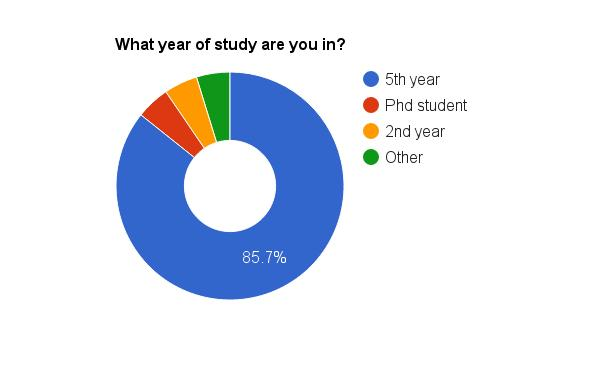
\includegraphics[width=1.5\textwidth]{results/year_of_study.jpg}}
        \caption{*}
        \label{fig:year-of-study}
    \end{subfigure}
    ~ %add desired spacing between images, e. g. ~, \quad, \qquad, \hfill etc.
      %(or a blank line to force the subfigure onto a new line)
    \hfill
    \begin{subfigure}[h]{0.45\textwidth}
        \centerline{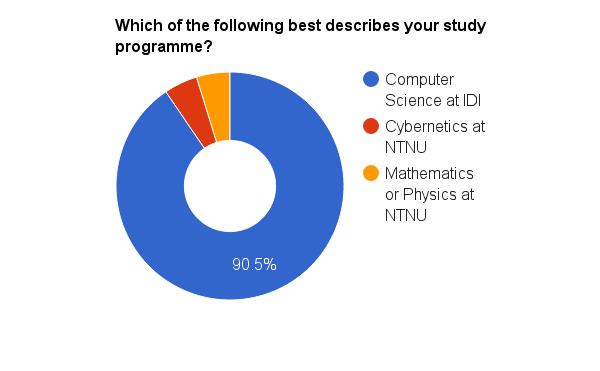
\includegraphics[width=1.5\textwidth]{results/study_programme.jpg}}
        \caption{*}
        \label{fig:study-programme}
    \end{subfigure}
    %add desired spacing between images, e. g. ~, \quad, \qquad, \hfill etc.
    %(or a blank line to force the subfigure onto a new line)

    %\hspace*{-1.5cm}
    \begin{subfigure}[h]{0.45\textwidth}
        \centerline{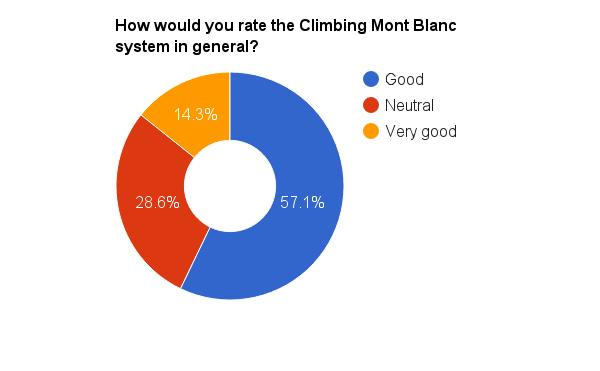
\includegraphics[width=1.5\textwidth]{results/general_cmb.jpg}}
        \caption{A1}
        \label{fig:cmb-general}
    \end{subfigure}
    \hfill
    \begin{subfigure}[h]{0.45\textwidth}
        \centerline{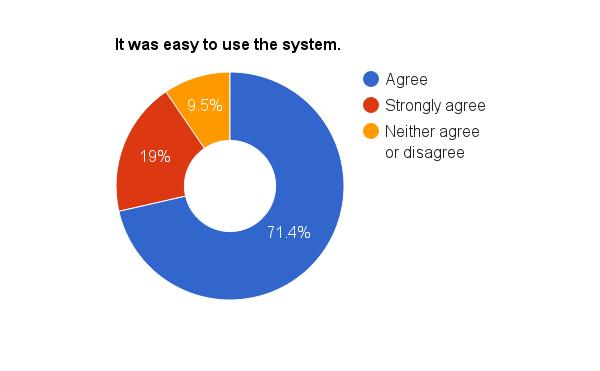
\includegraphics[width=1.5\textwidth]{results/easy_to_use.jpg}}
        \caption{B1}
        \label{fig:cmb-easy-use}
    \end{subfigure}
    \caption[]{Multiple Choice Results}
    \label{fig:multiplechoice}
\end{figure}


\begin{figure}
    \centering
    %\hspace*{-1.5cm}
    \begin{subfigure}[h]{0.45\textwidth}
        \centerline{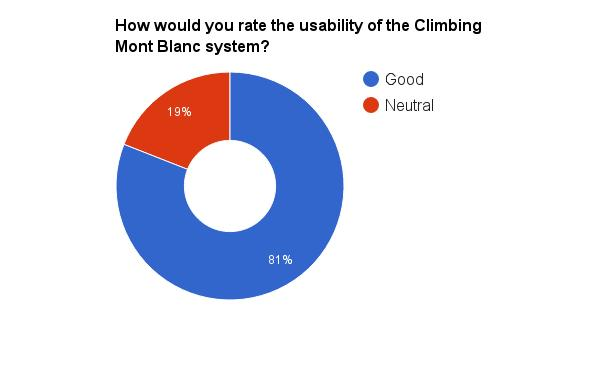
\includegraphics[width=1.5\textwidth]{results/usability_cmb.jpg}}
        \caption{A2}
        \label{fig:cmb-usability}
    \end{subfigure}
    ~ %add desired spacing between images, e. g. ~, \quad, \qquad, \hfill etc.
      %(or a blank line to force the subfigure onto a new line)
    \hfill
    \begin{subfigure}[h]{0.45\textwidth}
        \centerline{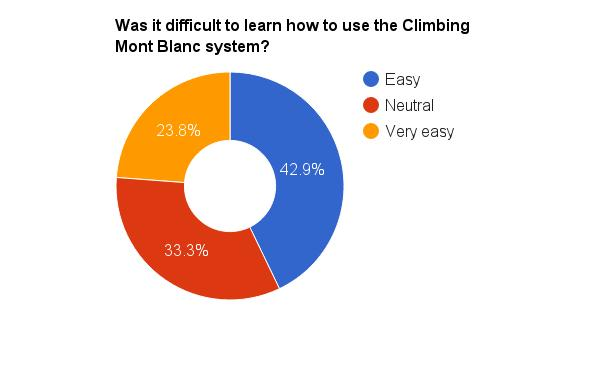
\includegraphics[width=1.5\textwidth]{results/learn_cmb.jpg}}
        \caption{C1}
        \label{fig:cmb-learn}
    \end{subfigure}

    %\hspace*{-1.5cm}
    \begin{subfigure}[h]{0.45\textwidth}
        \centerline{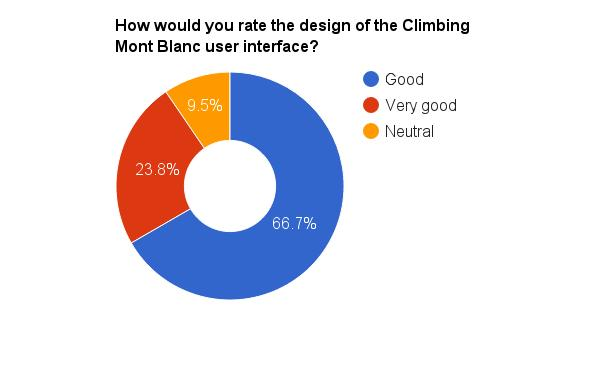
\includegraphics[width=1.5\textwidth]{results/design_cmb.jpg}}
        \caption{A3}
        \label{fig:cmb-design}
    \end{subfigure}
    ~ %add desired spacing between images, e. g. ~, \quad, \qquad, \hfill etc.
      %(or a blank line to force the subfigure onto a new line)
    \hfill
    \begin{subfigure}[h]{0.45\textwidth}
        \centerline{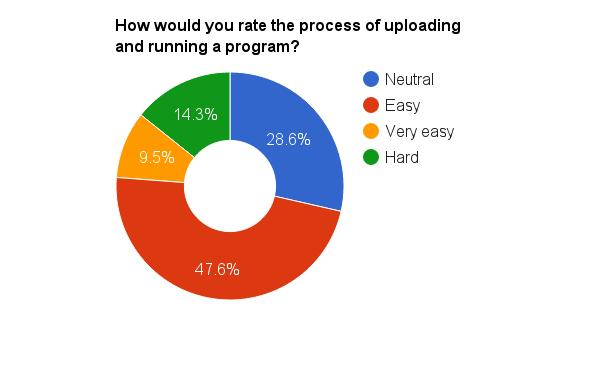
\includegraphics[width=1.5\textwidth]{results/submission_cmb.jpg}}
        \caption{C2}
        \label{fig:cmb-submission}
    \end{subfigure}
    \caption[]{Multiple Choice Results (continuation of Figure \ref{fig:multiplechoice})}
    \label{fig:multiplechoice1}
\end{figure}

\begin{figure}
    \centering
    %\hspace*{-1.5cm}
    \begin{subfigure}[h]{0.45\textwidth}
        \centerline{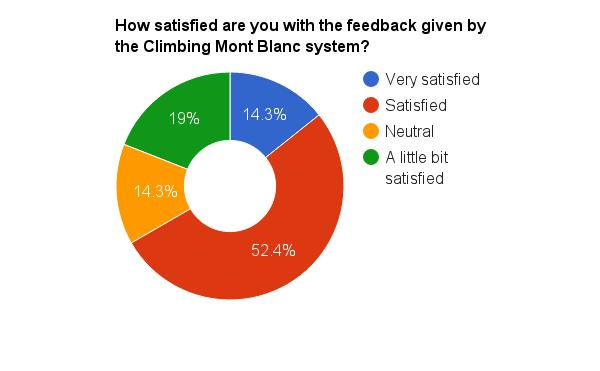
\includegraphics[width=1.5\textwidth]{results/feedback_cmb.jpg}}
        \caption{D1}
        \label{fig:cmb-feedback}
    \end{subfigure}
    \hfill
    \begin{subfigure}[h]{0.45\textwidth}
        \centerline{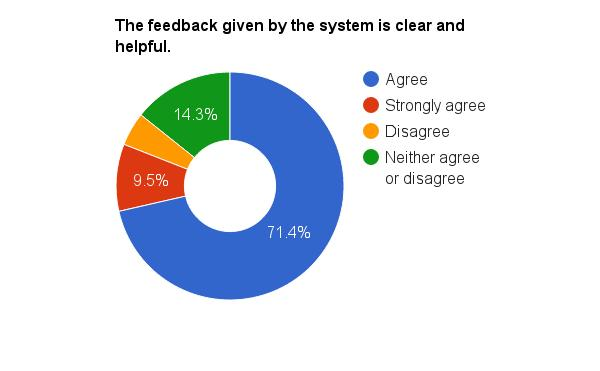
\includegraphics[width=1.5\textwidth]{results/clear_feedback_cmb.jpg}}
        \caption{B2}
        \label{fig:cmb-feedback-clear}
    \end{subfigure}

    %\hspace*{-1.5cm}
    \begin{subfigure}[h]{0.45\textwidth}
        \centerline{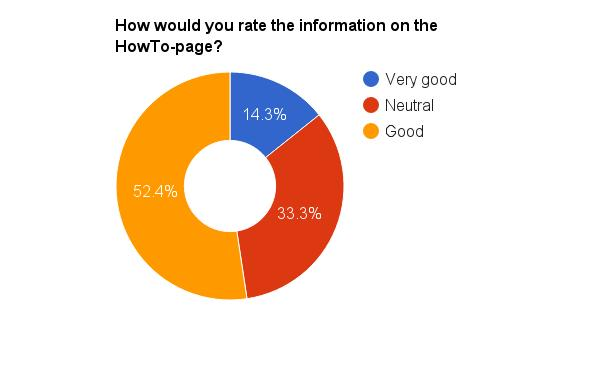
\includegraphics[width=1.5\textwidth]{results/howto_cmb.jpg}}
        \caption{A4}
        \label{fig:cmb-howto}
    \end{subfigure}
    \caption[]{Multiple Choice Results (continuation of Figure \ref{fig:multiplechoice1})}
    \label{fig:multiplechoice2}
\end{figure}

\section{TDT4200 User Study Results}
There were in total 37 students completing the survey. Figures \ref{fig:oldmultiplechoice} and \ref{fig:oldmultiplechoice1} shows the results of the multiple choice questions related to CMB. Some background information about the participants is also presented in Figure \ref{fig:oldsurvey-dist}. The Figure describes the distribution amongst the year of study and area of study. A summary of the feedback given in the textual based questions and feedback received in class is found below:

\begin{itemize}
\item Feedback given from the CMB system should be improved. Both regarding compilation errors and runtime errors.
\item The format and how to structure the zip to be uploaded was unclear. Would be nice to be able to upload single source files.
\item Submission of zip files from OSX did not work.
\item The delivery zip format through ItsLearning and CMB varied, which further lead to some confusion.
\item CMB had days with long run queue time.
\item Compilation and running of code should be done in one action.
\item One should be able to delete failed submissions as a user.
\item Running the same submission one more time should result in a new submission to the high score list, not an updated entry.
\item Sometimes, submissions that were chosen to be private were shown. The bug becomes present when sorting the highscore list on one of the other metrics.
\item The login procedure requires too many clicks.
\item CMB should support command line interface instead of the User Interface to compile and run programs.
\item Submissions is not visible accessing the problem page from a group view, only when accessing the problem from the public list of problems.
\item Expected compilation time and running time should be added, and also dynamic update the highscore list when runs have completed.
\item The submissions should display the lines of code and more information about the uploaded files.
\item The sorting of the highscore list should consider energy as a secondary priority next to running time when sorting the highscore list.
\item More languages should be supported.
\item Users should be able to specify compiler flags.
\item Detect content within the uploaded zip file.
\item CMB is a really good idea; you should try to improve it.
\item It needs some improvement, but, all in all, it is a good system.
\item Overall usability is good. But the system might need some overhaul of its components.
\end{itemize}

\begin{figure}
    \centering
    \hspace*{-1.5cm}
    \begin{subfigure}[h]{0.4\textwidth}
        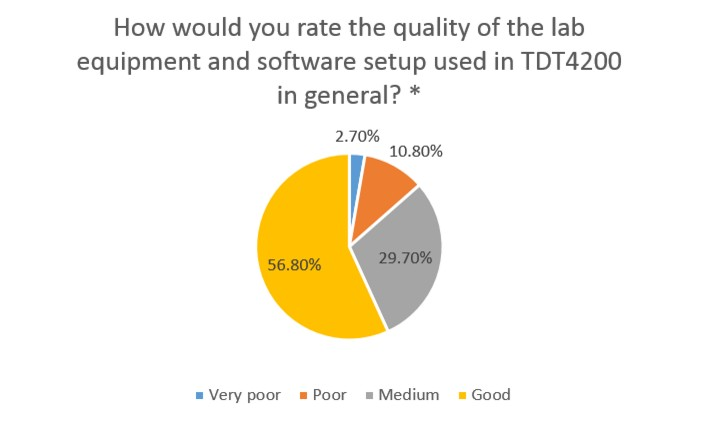
\includegraphics[width=1.5\textwidth, height=1.0\textwidth]{oldresults/equipment.jpg}
        \caption{}
        \label{fig:equipment}
    \end{subfigure}
    ~ %add desired spacing between images, e. g. ~, \quad, \qquad, \hfill etc.
      %(or a blank line to force the subfigure onto a new line)
    \hfill
    \begin{subfigure}[h]{0.4\textwidth}
        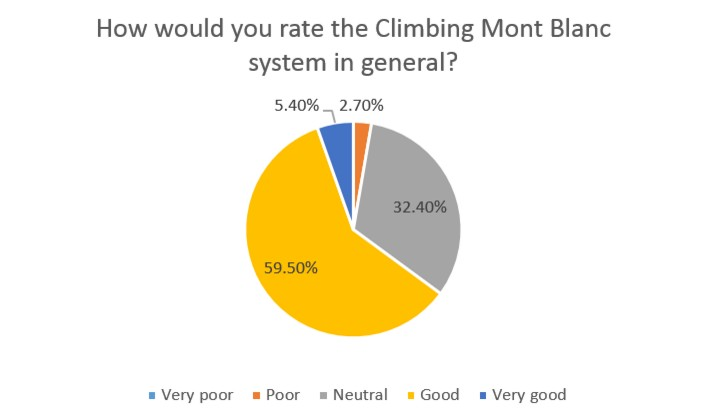
\includegraphics[width=1.5\textwidth, height=1.0\textwidth]{oldresults/cmb_general.jpg}
        \caption{}
        \label{fig:cmb-general}
    \end{subfigure}
    ~ %add desired spacing between images, e. g. ~, \quad, \qquad, \hfill etc.
    %(or a blank line to force the subfigure onto a new line)
    \hspace*{-1.5cm}
    \begin{subfigure}[h]{0.4\textwidth}
        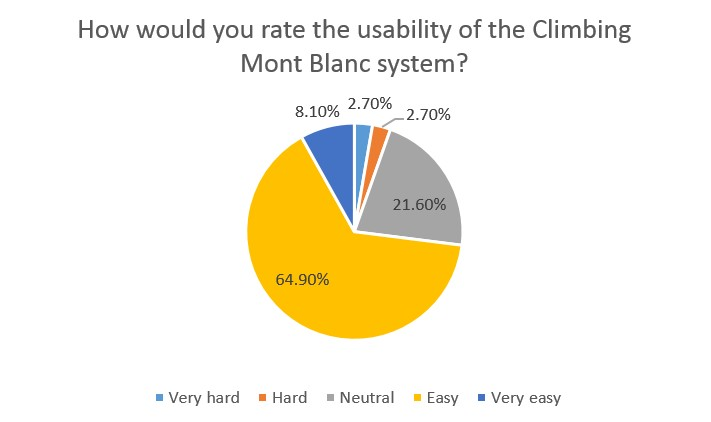
\includegraphics[width=1.5\textwidth, height=1.0\textwidth]{oldresults/cmb_usability.jpg}
        \caption{}
        \label{fig:cmb-usability}
    \end{subfigure}
    \hfill
    \begin{subfigure}[h]{0.4\textwidth}
        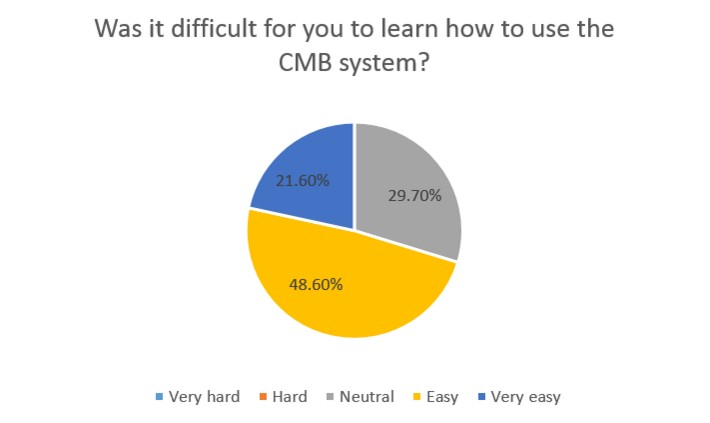
\includegraphics[width=1.5\textwidth, height=1.0\textwidth]{oldresults/cmb_learn.jpg}
        \caption{}
        \label{fig:cmb-learn}
    \end{subfigure}
    \hspace*{-1.2cm}
    \begin{subfigure}[h]{0.4\textwidth}
        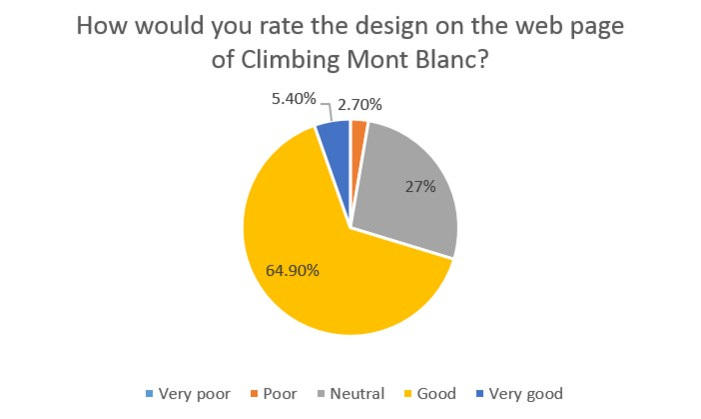
\includegraphics[width=1.5\textwidth, height=1.0\textwidth]{oldresults/cmb_design.jpg}
        \caption{}
        \label{fig:cmb-design}
    \end{subfigure}
    ~ %add desired spacing between images, e. g. ~, \quad, \qquad, \hfill etc.
      %(or a blank line to force the subfigure onto a new line)
    \hfill
    \begin{subfigure}[h]{0.4\textwidth}
        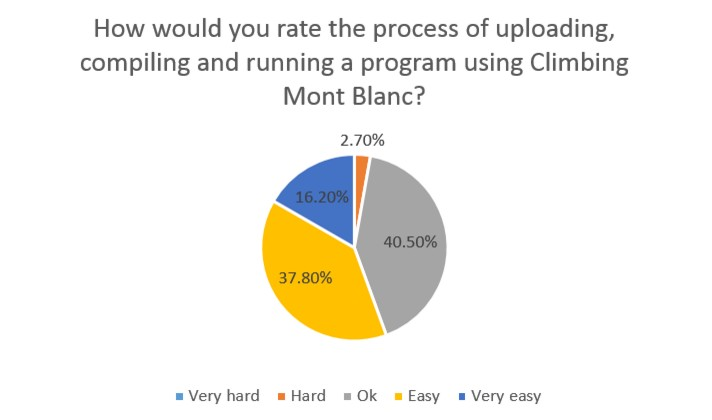
\includegraphics[width=1.5\textwidth, height=1.0\textwidth]{oldresults/cmb_tasks.jpg}
        \caption{}
        \label{fig:cmb-tasks}
    \end{subfigure}
    \caption[]{CMB Related Multiple Choice Results}
    \label{fig:oldmultiplechoice}
\end{figure}

\begin{figure}
    \hspace*{-1.5cm}
    \begin{subfigure}[h]{0.4\textwidth}
        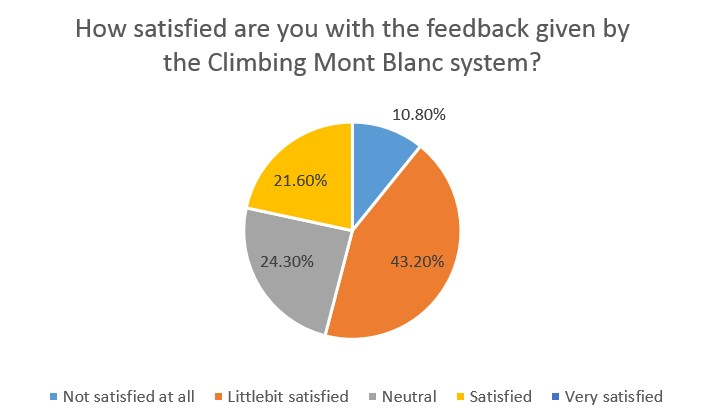
\includegraphics[width=1.5\textwidth, height=1.0\textwidth]{oldresults/cmb_feedback.jpg}
        \caption{}
        \label{fig:cmb-feedback}
    \end{subfigure}
    \hfill
    \begin{subfigure}[h]{0.4\textwidth}
        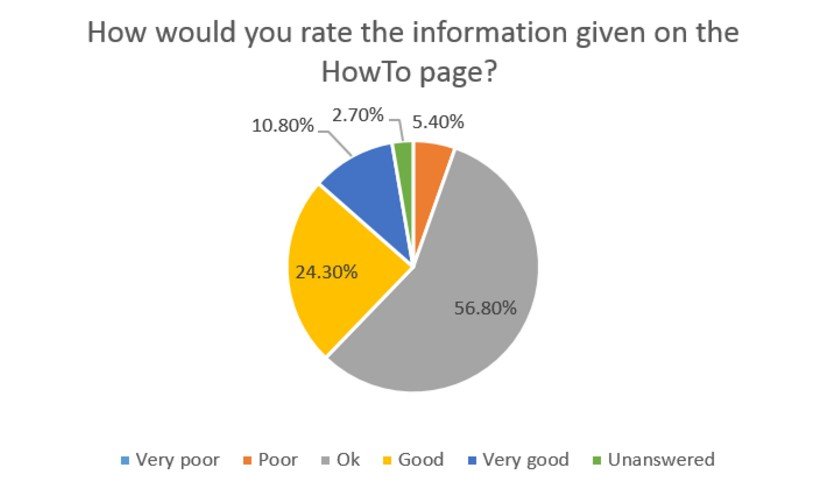
\includegraphics[width=1.5\textwidth, height=1.0\textwidth]{oldresults/cmb_howto.jpg}
        \caption{}
        \label{fig:cmb-howto}
    \end{subfigure}
    \caption[]{CMB Related Multiple Choice Results (continuation of \ref{fig:oldmultiplechoice})}
    \label{fig:oldmultiplechoice1}
\end{figure}

\begin{figure}
    \hspace*{-1.5cm}
    \begin{subfigure}[h]{0.4\textwidth}
        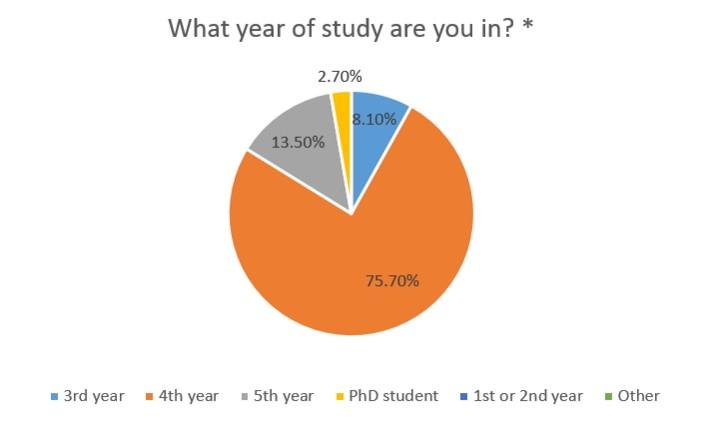
\includegraphics[width=1.5\textwidth, height=1.0\textwidth]{oldresults/participants.jpg}
        \caption{}
        \label{fig:distribution}
    \end{subfigure}
    \hfill
    \begin{subfigure}[h]{0.4\textwidth}
        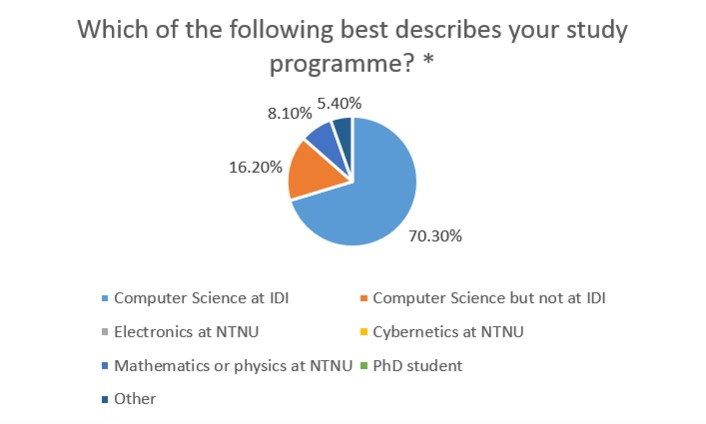
\includegraphics[width=1.5\textwidth, height=1.0\textwidth]{oldresults/distribution.jpg}
        \caption{}
        \label{fig:participants}
    \end{subfigure}
    \caption[]{Participant Distribution}
    \label{fig:oldsurvey-dist}
\end{figure}
